\documentclass[11pt]{article}

\usepackage{fullpage}
\usepackage{fourier}
\usepackage{euler}
\usepackage{amsmath}
\usepackage{graphicx}
\usepackage{xspace}
\usepackage{epigraph}
\usepackage{listings}
\usepackage{xcolor}
\usepackage{url}
\usepackage{hyperref}
\usepackage{soul}
\usepackage{floatflt}
\usepackage{pgfplots}
\usepackage{wrapfig}

\pgfplotsset{ compat=newest }

\usepackage{fancyhdr}
\pagestyle{fancy}
\fancyhf{}

\fancypagestyle{plain}{%
  \fancyhf{}
  \renewcommand{\headrulewidth}{0pt}
  \renewcommand{\footrulewidth}{0pt}
  \lfoot{\textcopyright{} 2021 Darrell Long}
  \rfoot{\thepage}
}

\pagestyle{plain}

\definecolor{codegreen}{rgb}{0,0.5,0}
\definecolor{codegray}{rgb}{0.5,0.5,0.5}
\definecolor{codepurple}{rgb}{0.58,0,0.82}

\lstloadlanguages{C,make,python,fortran}

\lstdefinestyle{c99}{
    morekeywords={bool, uint8_t, uint16_t, uint32_t, uint64_t, int8_t, int16_t, int32_t, int64_t},
    commentstyle=\color{codegreen},
    keywordstyle=\color{magenta},
    numberstyle=\tiny\color{codegray},
    identifierstyle=\color{blue},
    stringstyle=\color{codepurple},
    basicstyle=\ttfamily,
    breakatwhitespace=false,
    breaklines=true,
    captionpos=b,
    keepspaces=true,
    numbers=left,
    numbersep=5pt,
    showspaces=false,
    showstringspaces=false,
    showtabs=false,
    tabsize=4
}


\title{Assignment 3 \\ The Game of Life}
\author{Prof. Darrell Long \\ CSE 13S -- Winter 2021}
\date{Due: January 31$^\text{th}$ at 11:59\,pm}

\epigraphwidth=0.75\textwidth

\begin{document}\maketitle

\section{Introduction}
\epigraph{\emph{The last level of metaphor in the Alice books is this: that life, viewed
rationally and without illusion, appears to be a nonsense tale told by an idiot mathematician.}}{
---Martin Gardner}

John Horton Conway was an English mathematician active in the theory
of finite groups, knot theory, number theory, combinatorial game
theory, and coding theory. He also made contributions to many
branches of recreational mathematics, most notably in popular
culture for the invention of the cellular automaton called the
\emph{Game of Life}.

%\begin{wrapfigure}{r}{0.2\textwidth}
%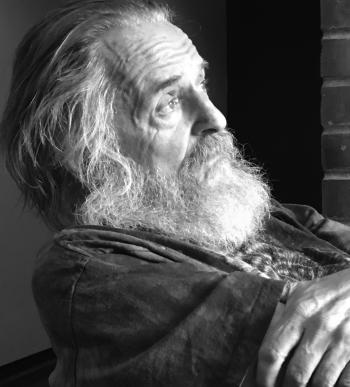
\includegraphics[width=0.2\textwidth]{images/Conway-kohn.jpg}
%\centerline{\small John Horton Conway}
%\end{wrapfigure}

Born and raised in Liverpool (home of the \emph{Beatles}), Conway spent the
first half of his career at the University of Cambridge before moving to the
United States, where he held the John von Neumann Chair at Princeton
University for the rest of his career. On 11 April 2020, at 82, he died of
complications from COVID-19.

Research on the Go end-game by Conway led to the original
definition and construction of the surreal numbers. Conway's
construction was introduced in Donald Knuth's 1974 book \emph{Surreal
Numbers: How Two Ex-Students Turned on to Pure Mathematics and Found
Total Happiness}. In his book, which takes the form of a dialogue,
Knuth coined the term \emph{Surreal Numbers} for what Conway had called
simply \emph{numbers}. Conway later adopted Knuth's term, and used
surreals for analyzing games in his 1976 book \emph{On Numbers and Games}.

\begin{wrapfigure}{l}{0.2\textwidth}

\includegraphics[width=0.2\textwidth]{images/CK.png}
\centerline{\small John Horton Conway}
\end{wrapfigure}

Conway first conceived The Game of Life in 1970 to describe how life can evolve
from an initial state. The concept builds on ideas that trace back to John von
Neumann\footnote{J. von Neumann and A. W. Burks, \emph{Theory of
self-reproducing automata}. Urbana, University of Illinois Press, 1960.} who was a
pioneer of early computing and from whom we get the von Neumann architecture that
we still use today.  Conways game involves a two-dimensional grid in which each
square cell interacts with its neighbors according to a simple set of rules. Over time,
these simple interactions give rise to surprising complexity.

Life, is a zero-player game, meaning that its evolution is
determined by its initial state, requiring no further input. One interacts with
the Game of Life by creating an initial configuration and observing how it
evolves. It is \emph{Turing complete} and can simulate a universal constructor or any
other Turing machine. Turing completeness means that for those who have yet to
study computability theory, the Game of Life can run \emph{any program} that can
be written for a computer.


\section{The Rules}
\epigraphwidth=0.5\textwidth
\epigraph{\emph{Our noblest hopes grow teeth and pursue us like tigers.}}
{---John Gardner, \emph{In the Suicide Mountains}}

The Game of Life should be played on a potentially \emph{infinite}, two-dimensional (2-D) grid of
cells that represents a \emph{universe}. Each cell has two possible states: it is
either \emph{dead} or \emph{alive}. The game progresses through
\emph{generations}, what some might call ``steps in time.'' There are only three rules
that determine the state of the universe after each generation:

\begin{enumerate}
  \item Any \emph{live} cell with two or three live neighbors \emph{survives}.
  \item Any \emph{dead} cell with exactly three live neighbors \emph{becomes a live cell}.
  \item All other cells die, either due to loneliness or overcrowding.
\end{enumerate}

Your task for this assignment is to implement the Game of Life in \textbf{C}.
The first hurdle is creating an abstraction for the universe in which the game
is played.


\section{The Universe}
\epigraph{\emph{Talking, talking. Spinning a web of words, pale walls of dreams, between myself and all I see.}}
{---John Gardner, \emph{Grendel}}

You will now write your first \emph{abstract data type},
commonly referred to as an \textbf{ADT}. This ADT will provide the abstraction
for a universe, a \emph{finite} 2-D grid of cells. Why not an infinite grid?
Because computers work in \emph{finite memory}. The following subsections will
walk you through the list of constructor, destructor, accessor, and manipulator
functions required for your ADT. You will be supplied \texttt{universe.h} (in the Resources repository), the
header file for the \texttt{Universe} ADT and you \textcolor{red}{\textbf{may not}} modify it.

\subsection{\texttt{Universe}}

The universe will be abstracted as a \texttt{struct} called \texttt{Universe}.
We will use a \texttt{typedef} to construct a new type, which you should treat
as opaque --- which means that you must pretend that you cannot manipulate it
directly. \textbf{C}, unlike some more modern languages, \emph{does not enforce opacity}.

Here, \texttt{universe.h} \emph{declares} the new type and \texttt{universe.c} \emph{defines} its concrete implementation.
Once again, \textcolor{red}{\textbf{you cannot modify universe.h}}

\begin{codelisting}{}
struct Universe {
    int rows;
    int cols;
    bool **grid;
    bool toroidal;
};
\end{codelisting}

An instance of a \texttt{Universe} must contain the following fields:
\texttt{rows}, \texttt{cols}, and a 2-D boolean grid, \texttt{grid}. Since there
are two states: \emph{alive} and \emph{dead}, then a natural choice for
representing the states is the \texttt{bool} type. A cell with the value
\texttt{false} in \texttt{grid} indicates that the cell is dead; the value
\texttt{true} indicates that the cell is alive. It is also possible for a
\texttt{Universe} to be \emph{toroidal}, which is indicated by the
\texttt{toroidal} field. \textcolor{red}{This \texttt{struct} definition must
be placed in the file \texttt{universe.c}.}


\subsection{\texttt{Universe *uv\_create(int rows, int cols, bool toroidal)}}

This is the constructor function that creates a \texttt{Universe}. The first two
parameters it accepts are the number of \texttt{rows} and \texttt{cols}, indicating the
dimensions of the underlying \emph{boolean} grid. The last parameter 
\texttt{toroidal} is a boolean. If the value of \texttt{toroidal} is
\texttt{true}, then the universe is \emph{toroidal}. The \emph{return type} of
this function is of type \texttt{Universe *}, meaning the function should return a
\emph{pointer} to a \texttt{Universe}. You will be using the \texttt{calloc()}
function from \texttt{<stdlib.h>} to dynamically allocate memory. 
For more information on \texttt{calloc()}, read \texttt{man calloc}.
Here is an example of allocating a matrix of \texttt{int}s:

\begin{codelisting}{}
int **matrix = (int **) calloc(rows, sizeof(int *));
for (int r = 0; r < rows; r += 1) {
    matrix[r] = (int *) calloc(cols, sizeof(int));
}
\end{codelisting}

Note that we first allocate a column of pointers  to rows, and then we allocate the actual rows.

For an example of a complete ADT constructor function, see the section on ADTs
in the course coding standards.


\subsection{\texttt{void uv\_delete(Universe *u)}}

This is the destructor function for a \texttt{Universe}. Simply put, it frees
any memory allocated for a \texttt{Universe} by the constructor function. Unlike
Java and Python, \textbf{C} is \emph{not} garbage collected. Not freeing
allocated memory by the end a program results in a \emph{memory leak}. Your
programs should be free of memory leaks. In the case of multilevel data
structures such as a \texttt{Universe}, we must free the inside first. Imagine
getting rid of a water bucket: you should dump out the water before scrapping
the bucket. Use \texttt{valgrind} to check for memory leaks -- the graders will too!


\subsection{\texttt{int uv\_rows(Universe *u)}}

Since we will be using \texttt{typedef} to create \emph{opaque} data types, we
need functions to access fields of a data type. These functions are called
\emph{accessor} functions. An opaque data type means that users do not need to know its
implementation outside of the implementation itself. This means that it is
incorrect to have \texttt{u->rows} outside of \texttt{universe.c} as it violates
opacity. 
This function returns the number of rows in the specified \texttt{Universe} (it is possible, but only inside \texttt{universe.c}).


\subsection{\texttt{int uv\_cols(Universe *u)}}

Like \texttt{uv\_rows()}, this function is an accessor function and returns the
number of columns in the specified \texttt{Universe}.


\subsection{\texttt{void uv\_live\_cell(Universe *u, int r, int c)}}

The need for \emph{manipulator} functions follows the rationale behind the need
for accessor functions: we need some way to alter fields of a data type. This
function simply marks the cell at row \texttt{r} and column \texttt{c} as live.
If the specified row and column lie outside the bounds of the universe, nothing
changes. Since we are using \emph{bool}, we assume that \emph{true} means live
and \emph{false} means dead.


\subsection{\texttt{void uv\_dead\_cell(Universe *u, int r, int c)}}

This function marks the cell at row \texttt{r} and column \texttt{c} as \emph{dead}.
Like in \texttt{uv\_live\_cell()}, if the row and column are out-of-bounds,
nothing is changed.


\subsection{\texttt{bool uv\_get\_cell(Universe *u, int r, int c)}}

This function returns the value of the cell at row
\texttt{r} and column \texttt{c}. If the row and column are out-of-bounds,
\texttt{false} is returned. Again, \emph{true} means the cell is live.


\subsection{\texttt{bool uv\_populate(Universe *u, FILE *infile)}}

This function will populate the \texttt{Universe} with row-column pairs read in
from \texttt{infile}. This function will require the use of \texttt{<stdio.h>}
since \texttt{infile} is a \texttt{FILE *} (\texttt{FILE} is defined in the
\texttt{<stdio.h>} library). The necessary \emph{include} will be supplied in
\texttt{universe.h} for you. A valid input file that could be fed into your
program would be:

\begin{codelisting}{}
36 65
2 32
3 30
\end{codelisting}

The first line of a valid input file for your program consists of the number of
rows followed by the number of columns of the universe. Each subsequent line
is the row and column of a live cell. You will want a loop that makes calls to
\texttt{fscanf()} to read in all the row-column pairs in order to populate the
universe. If a pair lies beyond the dimensions of the universe, and return \texttt{false} to indicate that the universe failed to
be populated. Return \texttt{true} if the universe is successfully populated. Failure
to populate the universe should cause the game to fail with an error message.

\textcolor{red}{\emph{Do not} print in functions if you can avoid it -- unless that is their job!}


\subsection{\texttt{int uv\_census(Universe *u, int r, int c)}}

\begin{wrapfigure}{r}{0.125\textwidth}
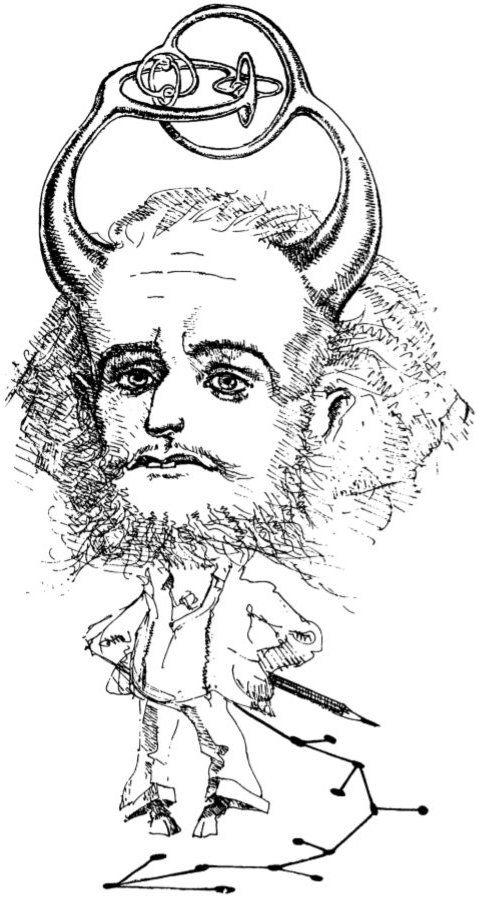
\includegraphics[width=0.125\textwidth]{images/horns.jpg}
\end{wrapfigure}

When we consider our universe, a flat universe is simply a grid.  Ideally
in the Game of Life, that extends to infinity in the $\pm x$ and $\pm y$
directions. Since we cannot have an infinite grid, we are left with a choice: we
can either, as the Flat Earthers believe, have things fall off the edge or come
up with some other solution. Our solution will be to treat the finite grid as a
flat Earth or as a
\emph{torus}. An example of a torus can be constructed by taking a rectangular
strip of flexible material, for example, a rubber sheet, and joining the top
edge to the bottom edge, and the left edge to the right edge, without any
half-twists.

It requires some reflection, but if you think about you will see
that a torus is any topological space that is topologically equivalent
to a torus. A coffee cup and a doughnut are both topological tori.

\begin{center}
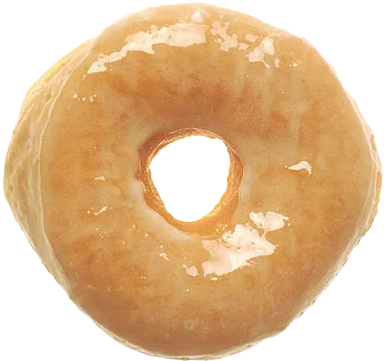
\includegraphics[width=1.7in]{images/donut.png}\hfil

\includegraphics[width=2in]{images/torus.png}\hfil

\includegraphics[width=1.7in]{images/cup.png}
\end{center}

In the realm of real numbers, the parametric equation of a ring torus is:
\begin{align*}
x(\theta, \phi) & = (R + r \cos \theta) \cos \phi \\
y(\theta, \phi) & = (R + r \cos \theta) \sin \phi \\
z(\theta, \phi) & = r \sin \theta
\end{align*}

\noindent where $\theta$, and $\phi$ are angles which make a full circle, so that their
values start and end at the same point, $R$ is the distance from the center of
the tube to the center of the torus, and $r$ is the radius of the tube.  Our
torus is finite and discrete: in other words, assuming a square grid $G_{n,n}$
indexed from $0, \ldots, n-1$ (because we are Computer Scientists), the right
edge of the grid $G_{i, n-1}$ is connected (succeeded by) $G_{i, 0}$, and the
bottom edge of the grid $G_{n-1, i}$ is connected to $G_{0, i}$.
In other words, \emph{successor} and \emph{predecessor} are calculated using \emph{modular
arithmetic} if the universe is a torus, which you have seen these functions before.

This function returns the number of \emph{live neighbors} adjacent to the cell
at row \texttt{r} and column \texttt{c}. If the universe is flat, or
non-toroidal, then you should only consider the \emph{valid} neighbors for the count.
If the universe is toroidal, then all neighbors are valid: you simply wrap to
the other side. \textcolor{red}{Tip: you should calculate the row and column for
each neighbor and apply modular arithmetic if the universe is toroidal.}


\subsection{\texttt{void uv\_print(Universe *u, FILE *outfile)}}

This functions prints out the universe to \texttt{outfile}. A live cell is
indicated with the character `\texttt{o}' (a lowercase O) and a dead cell is
indicated with the character `\texttt{.}' (a period). You will want to use
either \texttt{fputc()} or \texttt{fprintf()} to print to the specified
\texttt{outfile}. Since you cannot print a torus, you will always print out the
flattened universe.


\section{Controlling the Cursor}
\epigraphwidth=0.6\textwidth
\epigraph{\emph{An orphan's curse would drag to hell \\
A spirit from on high; \\
But oh! more horrible than that \\
Is the curse in a dead man's eye! \\
Seven days, seven nights, I saw that curse, \\
And yet I could not die.}}{---Samuel Taylor Coleridge, \emph{The Rime of the Ancient Mariner}}

\texttt{ncurses} is a programming library used to develop text-based user
interfaces. It is used in vi (vim, neovim), emacs and many other programs.
You will use this library to display the state of the universe after
each evolution. Here is some code that showcases moving an `\texttt{o}'
horizontally across the screen:

\begin{codelisting}{Short \texttt{ncurses} example.}
#include <ncurses.h>
#include <unistd.h> // For usleep().

#define ROW 0
#define DELAY 50000

int main(void) {
    initscr(); // Initialize the screen.
    curs_set(FALSE); // Hide the cursor.
    for (int col = 0; col < 40; col += 1) {
        clear(); // Clear the window.
        mvprintw(ROW, col, "o"); // Displays "o".
        refresh(); // Refresh the window.
        usleep(DELAY); // Sleep for 50000 microseconds.
    }
    endwin(); // Close the screen.
    return 0;
}
\end{codelisting}

To test this code snippet out, place it in \texttt{example.c} and compile it
with the command:

\begin{lstlisting}[style=bashstyle]
  $ clang -o example example.c -lncurses
\end{lstlisting}

The \texttt{-lncurses} at the end serves to \emph{link} the \texttt{ncurses}
library. Linked libraries should always be linked at the end. Why? \textsc{Unix}
links binaries from left to right. When an \emph{undefined} reference is
encountered, it is expected to be defined \emph{later}. An \emph{unreferenced} item is
ignored, so if you list the library first, it will be unreferenced and is thus
ignored.


\section{Command-line Options}
\epigraphwidth=0.6\textwidth
\epigraph{\emph{A few dud universes can really clutter up your basement.}}{Neal Stephenson, \emph{In the Beginning\ldots Was the Command Line}}

Your program should accept the following command-line options:

\begin{itemize}
  \item \texttt{-t}\ : Specify that the Game of Life is to be played on a \emph{toroidal}
    universe.
  \item \texttt{-s}\ : Silence \texttt{ncurses}. Enabling this option means
    that nothing should be displayed by \texttt{ncurses}.
  \item \texttt{-n} \emph{generations}\ : Specify the number of generations that the
    universe goes through. The default number of generations is 100.
  \item \texttt{-i} \emph{input}\ : Specify the input file to read in order to populate
    the universe. By default the input should be \texttt{stdin}.
  \item \texttt{-o} \emph{output}\ : Specify the output file to print the final state
    of the universe to. By default the output should be \texttt{stdout}.
\end{itemize}


\section{Specifics}
\epigraphwidth=0.4\textwidth
\epigraph{\emph{Jehosaphat the mongrel cat \\
Jumped off the roof today \\
Some would say he fell but I could tell \\
He did himself away}}{---John Prine, \emph{Living in the Future}}

Here are the specifics for your assignment implementation.

\begin{enumerate}
  \item Parse the command-line options by looping calls to \texttt{getopt()}.
    This should be similar to what you did in assignment 2.
  \item Use an initial call to \texttt{fscanf()} to read the number of rows and columns of
    the universe you will be populating from the specified input.
  \item Create \emph{two} universes using the dimensions that were obtained using \texttt{fscanf()}. Mark
    the universes toroidal if the \texttt{-t} option was specified. We will
    refer to these universes as universe $A$ and universe $B$.
  \item Populate universe $A$ using \texttt{uv\_populate()} with the remainder of the
    input.
  \item Setup the \texttt{ncurses} screen, as show by the example in \S 4.
  \item For each generation up to the set number of generations:
    \begin{enumerate}
      \item If \texttt{ncurses} isn't silenced by the \texttt{-s} option, clear
        the screen, display universe $A$, refresh the screen, then sleep for 50000
        microseconds.
      \item Perform one generation. This means taking a census of each cell in
        universe $A$ and either setting or clearing the corresponding cell in
        universe $B$, based off the 3 rules discussed in \S 2.
      \item Swap the universes. Think of universe $A$ as the current state of the
        universe and universe $B$ as the next state of the universe. To update the
        universe then, we simply have to swap $A$ and $B$. \textcolor{red}{Hint:
        swapping \emph{pointers} is much like swapping integers.}
    \end{enumerate}
  \item Close the screen with \texttt{endwin()}.
  \item Output universe $A$ to the specified file using \texttt{uv\_print()}.
    This is what you will be graded on. We will know if you properly
    evolved your universe for the set number of generations by comparing your output
    to that of the supplied program.
\end{enumerate}


\section{Deliverables}
\epigraphwidth=0.4\textwidth
\epigraph{\emph{It is such a sweet temptation \\
It gives such grief relief \\
It is such a false sensation \\
How come that's so hard to believe?}}{---Ray Wylie Hubbard, \emph{Loco Gringo's Lament}}

\noindent You will need to turn in:
\begin{enumerate}
  \item \texttt{life.c}: This file will contain your implementation of the Game
    of Life.
  \item \texttt{universe.c} should contain the
    implementation of the \texttt{Universe} ADT.
  \item \texttt{universe.h} should
    contain the definitions. You will be supplied \texttt{universe.h} and
    \emph{may not} modify it.
  \item \texttt{Makefile}: This is a file that will allow the grader to type
    \texttt{make} to build and run your program. Your \texttt{Makefile}
    \emph{must} support the following targets:
    \begin{itemize}
      \item \texttt{all}: Builds your program.
      \item \texttt{clean}: Removes any compiler-generated files.
      \item \texttt{format}: Formats any source or header files with the
        course-supplied \texttt{clang-format} file.
    \end{itemize}
  \item \texttt{README.md}: This must be in \emph{Markdown}. This must describe
    how to build and run your program. It should also describe the command-line
    options that your program accepts.
  \item \texttt{DESIGN.pdf}: This \emph{must} be in PDF\@. The design document
    should describe the purpose of your program and communicate its overall
    design with enough detail such that a sufficiently knowledgeable programmer
    would be able to replicate your implementation.  \textcolor{red}{This does
    not mean copying your entire program in verbatim.} You should instead
    describe how your program works with supporting pseudocode.
    \textcolor{red}{\textbf{C} code is \textbf{not} considered pseudocode. You
    \emph{must} push \texttt{DESIGN.pdf} \textbf{before} you push \emph{any} code.}
\end{enumerate}

We will provide an example of both \texttt{README.md} and \texttt{DESIGN.pdf} for your reference.


\section{Submission}
\epigraphwidth=0.6\textwidth
\epigraph{\emph{People say that if you're still angry at 52, you're not an angry young man, just a grumpy old git.}}{Paul Weller}

To submit your assignment through \texttt{git}, refer to the steps shown in
\texttt{asgn0} Remember: \emph{add, commit,} and \emph{push}!
\textcolor{red}{Your assignment is turned in \emph{only} after you have pushed.
If you forget to push, you have not turned in your assignment and you will get a
\emph{zero}. ``I forgot to push'' is not a valid excuse. It is \emph{highly}
recommended to commit and push your changes \emph{often}.}

We will provide you with an \emph{Ubuntu 20.04} binary of our implementation.
Your code must produce \emph{exactly} the same output for \emph{all} inputs in
order to receive full credit. You can use the Linux \texttt{diff} command to 
compare results.


\section{Supplemental Readings}

\epigraph{\emph{The more that you read, the more things you will know. The
more that you learn, the more places you'll go.}}{---Dr.\ Seuss}\noindent

\begin{itemize}
  \item \textit{The C Programming Language} by Kernighan \& Ritchie
    \begin{itemize}
      \item Chapter 3 \S 3.4--3.7
      \item Chapter 4 \S 4.1 \& 4.2 \& 4.5
      \item Chapter 5 \S 5.1--5.2 \& 5.10
      \item Chapter 6 \S 6.1--6.5 \& 6.7
      \item Chapter 7 \S 7.2 \& 7.5
      \item Appendix B \S B5
    \end{itemize}
    
  \item \textit{The Kollected Kode Vicious } by George V. Neville-Neil
  \begin{itemize}
      \item Chapter 1 \S 1.3, \& 1.5-1.7
  \end{itemize}
  
  \item  Martin Martin,
    \href{https://web.stanford.edu/class/sts145/Library/life.pdf}{\emph{Mathematical
    Games --- The Fantastic Combinations of John Conway's New Solitaire Game
`Life',}} Scientific American (223): 120--123 (October 1970).
\end{itemize}
\end{document}

